\section{Contexto}

\subsection{El centro}

El Centro Mexicano para la Producción más Límpia (en adelante, CMPL) es una instancia del Instituto Politécnico Nacional que se dedica a la investigación y elaboración de procesos de producción más limpia. El CMPL, como dice en su página web, “es integrante de la red mundial de centros de producción más límpia y de la red latinoamericana de producción más limpia, promovidas por la Organización de las Naciones Unidas para el Desarrollo Industrial (ONUDI) y el Programa de las Naciones Unidas para el Medio Ambiente (PNUMA). Cuenta con 13 años de experiencia realizando trabajo técnico para la industria nacional atendiendo sectores como alimentos, petroquímicos, cementeros, galvanoplastia y embotelladoras, por mencionar algunos. Los servicios que ofrece el CMPL son: diagnóstico en producción más limpia y eficiencia energética, diplomados a distancia, presenciales y Maestría en Producción Más Limpia, realización de proyectos de mecanismo de desarrollo limpio, planes de manejo de residuos y análisis de químicos” [1].\\

\subsection{Actividades}

El CMPL consta de varios departamentos, dentro de los cuales  se encuentra el Departamento de Sistemas y Banco de Datos encargado de sistematizar, desarrollar y automatizar los procesos y/o actividades del CMPL. Así mismo también se encuentra Oficialía de Partes que se encarga de llevar el registro y seguimiento a los asuntos que ingresan mediante un documento (oficios) al centro y la Dirección que es la encargada de turnar, dar seguimiento y atender cada asunto según sea el caso. \\
Dichas actividades se dividen en tres procesos que son: \\

\begin{itemize}
	\item Registro de documentos.
	\item Atención de documentos.
	\item Respuesta de documentos.
\end{itemize}

\subsubsection{Registrar Documento}

%%%%% PROCESO DE DOCUMENTOS %%%%%
	\begin{figure}[htbp!]
		\centering
			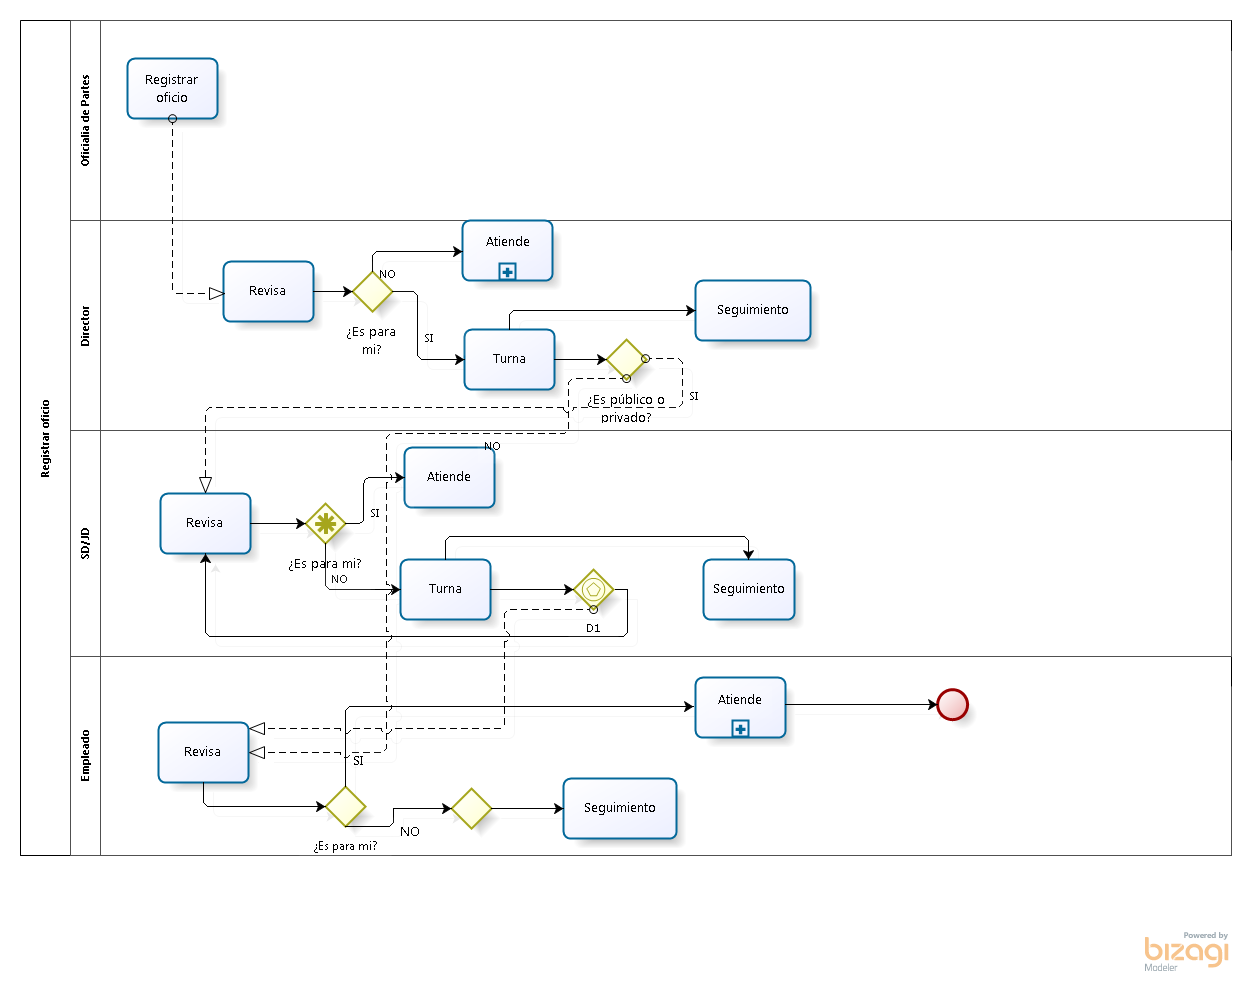
\includegraphics[width=0.7\textwidth]{images/procesoregistro}
		\caption{Proceso Registro de Documentos.}
	\end{figure}

\subsubsection{Atención de Documento}	

	\begin{figure}
		\centering
			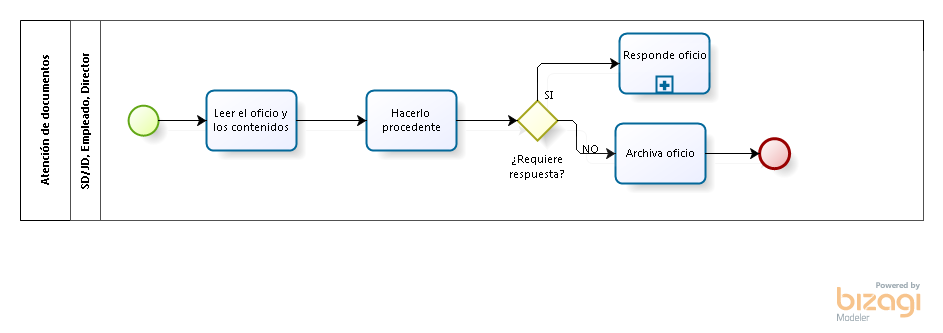
\includegraphics[width=0.8\textwidth]{images/procesoatencion}
		\caption{Proceso Atención de Documentos.}
	\end{figure}

\subsubsection{Respuesta de Documento}	

	\begin{figure}
		\centering
			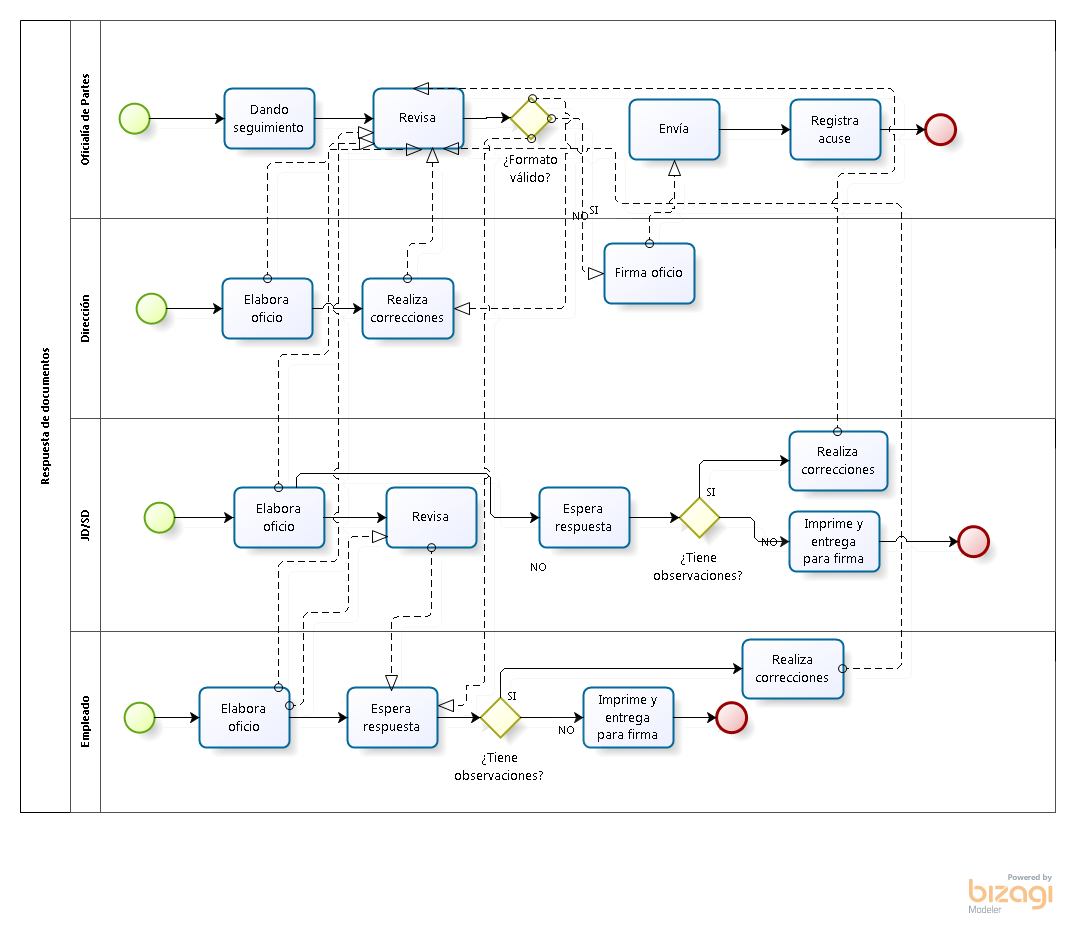
\includegraphics[width=0.7\textwidth]{images/procesorespuesta}
		\caption{Proceso Respuesta de Documentos.}
	\end{figure}
%%%%%%%%%%%%%%%%%%%%%%%%%%%%%%%%%%%%%%%%%%%%%%%%%%%%%%%%%%%%%%%%%%%%%%%%%%%%%%%%%%

\subsection{Normatividad}	

Existen ciertas normas establecidas a nivel mundial para toda empresa que le permiten tener un mejor trato con el medio ambiente, orientando el uso de las tecnologías de la información para reducir costos de producción y uso de materiales como papel, reduciendo considerablemente su huella ecológica. El CMPL, al ser una institución para la producción más limpia, hace uso de dos estándares que son fundamentales para cualquier centro de investigación o empresa de su índole, particularmente, las normas ISO 9001:2008 e ISO 14000.\\

\subsubsection{ISO 9001:2008}

La norma ISO 9001:2008 determina los requisitos para un Sistema de Gestión de la Calidad (SGC), que pueden utilizarse para su aplicación interna por las organizaciones, sin importar si el producto o servicio lo brinda una organización pública o empresa privada, cualquiera que sea su tamaño, para su certificación o con fines contractuales.\\

Capítulo 4 Sistema de gestión: contiene los requisitos generales y los requisitos para gestionar la documentación.\\

\subsubsection{ISO 14000}
La norma ISO 14000 expresa cómo establecer un Sistema de Gestión Ambiental (SGA) efectivo, va enfocada a cualquier organización, de cualquier tamaño o sector, que esté buscando reducir los impactos en el ambiente y cumplir con la legislación en materia ambiental. Es un conjunto de documentos de gestión ambiental que, una vez implantados, afectará todos los aspectos de la gestión de una organización en sus responsabilidades ambientales y ayudará a las organizaciones a tratar sistemáticamente asuntos ambientales, con el fin de mejorar el comportamiento ambiental y las oportunidades de beneficio económico.
